\documentclass[uplatex, 12pt, dvipdfmx]{jsreport}
\usepackage[ipaex, unicode]{pxchfon}
\usepackage{amsmath}
\usepackage{amsfonts}
\usepackage{amssymb}
\usepackage{color}
\usepackage{tikz}

\newtheorem{thm}{定理}
\newtheorem{dfn}[thm]{定義}
\newtheorem{lem}[thm]{補題}
\newtheorem{prop}[thm]{命題}

\newcommand{\mfa}{\mathfrak{a}}
\newcommand{\mfb}{\mathfrak{b}}
\newcommand{\mfp}{\mathfrak{p}}
\newcommand{\mfq}{\mathfrak{q}}

\newcommand{\mcF}{\mathcal{F}}
\newcommand{\mcG}{\mathcal{G}}
\newcommand{\mcH}{\mathcal{H}}


\title{代数幾何学まとめノート}
\date{}

\begin{document}

\maketitle

\chapter{可換環}

\section{可換環}
\begin{dfn}
アーベル群 A が(単位的)\textbf{可換環}であるとは、
\textbf{積}と呼ばれる写像 $A \times A \to A$, $a, b \mapsto ab, \text{where}, a, b \in A$
を備えており、以下の公理を満たすときをいう: \\

任意の $a, b, c \in A$ について
\begin{enumerate}
    \item ab = ba
    \item (ab)c = a(bc)
    \item (a + b)c = ac + bc
    \item 1a = a
\end{enumerate}
ここで、$1 \in a$ を $A$ の単位元という。
\end{dfn}
以降、単に環といったら単位的可換環のことを意味すると約束する。

\begin{dfn}
    環 $A$ から $B$ への写像 $\phi: A \to B$ が\textbf{環準同型写像}であるとは、次の性質を満たすときをいう:
    \begin{enumerate}
        \item $\phi(a + b) = \phi(a) + \phi(b)$
        \item $\phi(ab) = \phi(a)\phi(b)$
        \item $\phi(1) = 1$
    \end{enumerate}
\end{dfn}

\begin{dfn}
    環 $A$ の部分集合 $\mfa$ が\textbf{イデアル}であるとは、$\mfa$ が次の性質を満たすときをいう。
    \begin{enumerate}
        \item $\mfa$は加法に関して部分群である。すなわち
        \begin{enumerate}
            \item $0 \in \mfa$
            \item $\forall a \in \mfa, -a \in \mfa$
            \item $\forall a, \forall b \in \mfa$, $a + b \in \mfa$
        \end{enumerate}
        \item $\forall a \in \mfa, \forall x \in A$, $ax \in A$.
    \end{enumerate}
\end{dfn}

\begin{dfn}
    環 $A$ のイデアル $\mfp$ が\textbf{素イデアル}であるとは、$\mfp$ が次の性質を満たすときをいう。
    \[
        p, q \in A \text{について、\ } pq \in \mfp \text{ならば} p \in \mfp \text{または} q \in \mfp.
    \]
\end{dfn}

\begin{dfn}
    (Wikipedia) 拡大体の{\bf 超越次数}とは、体の拡大$L/K$の大きさのある種のかなり粗いはかり方である。
    きちんと言えば、$K$上代数的に独立な$L$の部分集合の最も大きい濃度として定義される。
\end{dfn}

\begin{dfn}
体 $k$ の超越次数1の有限生成拡大体$K$を{\bf 1次元関数体と呼ぶ}。

\textcolor{red}{ここでは$K$として$k$上の1変数有理関数体$k(X)$を思い浮かべておけばよいはず。}
\end{dfn}

$K$ を $k$ 上の1次元関数体とする。
$C_K$ を $K/k$ の DVR すべてのなす集合とする。$C_K$の元を点とも呼ぶ。
\begin{center}
    $C_K \ni P \leftrightarrow R_P$ ($P$ に対応するDVR).
\end{center}

\begin{dfn}
    {\bf 抽象非特異曲線}とは $K$ を $k$ 上の1次元関数体として、開部分集合 $U \subseteq C_K$ である。
    ただし $U$ には誘導位相を与え、開部分集合上の正則関数の概念を $C_K$ の場合から定める。
\end{dfn}

\chapter{層}

\begin{dfn}
    $X$ を位相空間とする。$X$ 上の\textbf{前層} $\mcF$とは以下のようなデータである。
    \begin{enumerate}
        \item $X$ の各開集合 $U$ に対してアーベル群 $\mcF(U)$ が定まっている。
        \item $X$ の開集合 $U, V$ で、$V \subseteq U$ となるペアについてアーベル群の準同型写像
        $\rho_{UV}: \mcF(U) \to \mcF(V)$ が定まっている。 これを\textbf{制限写像}と呼ぶ。
    \end{enumerate}
    ただしこれらは以下の条件を満たすものとする:
    \begin{itemize}
        \item 空集合 $\emptyset$ に対しては $\mcF(\emptyset) = 0$ (自明なアーベル群)。
        \item $\rho_{UU}: \mcF(U) \to \mcF(U)$ は恒等写像。
        \item $X$ の開集合 $W \subseteq V \subseteq U$に対して、$\rho_{UW} = \rho_{VW}\circ\rho_{UV}$.
    \end{itemize}
\end{dfn}

$s \in \mcF(U)$ に対して $\rho_{UV}(s)$ を $s|_V$ と書くこともある。

\begin{dfn}{(層の茎と芽)\textcolor{red}{順極限の定義をする。もっとわかりやすく書く。}}
    $\mcF$ を $X$ 上の前層とし、$P$ を $X$ 上の点とする。$\mcF$ の $P$ における\textbf{茎} $\mcF_P$ を、
    $P$ を含む全ての開集合 $U$ に対する群 $\mcF(U)$ と制限写像 $\rho$ がなす順系に関する順極限と定義する。
    茎 $\mcF_P$ の元を点 $P$ における $\mcF$ の切断の\textbf{芽}という。
\end{dfn}

\begin{dfn}
    位相空間$X$の上の前層$\mcF$がさらに次の条件を満たすとき$\mcF$を\textbf{層}という。
    \begin{enumerate}
        \setcounter{enumi}{2}
        \item (局所性)$X$の任意の開集合$U$とその開被覆$\{V_i\}$に対して、
              $s \in \mcF(U)$ がすべての $i$ について $s|_{V_i} = 0$ を満たすならば $s = 0$.
        \item (貼り合わせ条件)各 $i$ について $s_i \in \mcF(V_i)$ があり、
              $s_i|_{V_i \cap V_j} = s_j|_{V_i \cap V_j}$ を満たすならば、ある $s \in \mcF(U)$
              が存在して、$s_i = s|_{V_i}$ となる。
    \end{enumerate}
\end{dfn}


\begin{dfn}{(前層の射)}
    $\mcF$, $\mcG$ を $X$ 上の前層とするとき、それらの間の射 $\phi: \mcF \to \mcG$ とは
    各開集合 $U \subset X$ に対するアーベル群の射 (= 準同型写像) $\phi(U): \mcF(U) \to \mcG(U)$ から
    なるもので、各 $\phi(U)$ が制限写像と可換になるものである。

    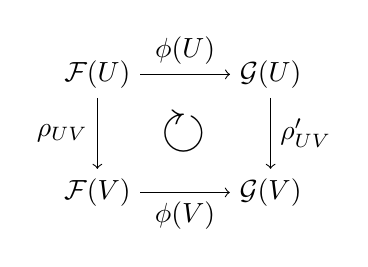
\begin{tikzpicture}[auto]
        \node (FU) at (0, 1.5) {$\mcF(U)$}; \node (GU) at (2.2, 1.5) {$\mcG(U)$};
        \node (FV) at (0, 0) {$\mcF(V)$};   \node (GV) at (2.2, 0) {$\mcG(V)$};
        \node (F) at (1.1, 0.75) {\huge$\circlearrowright$};
        \draw[->] (FU) to node {$\phi(U)$} (GU);
        \draw[->] (FV) to node[swap] {$\phi(V)$} (GV);
        \draw[->] (FU) to node[swap] {$\rho_{UV}$} (FV);
        \draw[->] (GU) to node {$\rho'_{UV}$} (GV);
    \end{tikzpicture}
\end{dfn}



\begin{dfn}{(前層に付随する層)}
    $X$ 上の前層 $\mcF$ が与えられたときに、それから$X$上の層 $\mcF^+$ を構成することができる:

    $X$ の各開集合 $U$ に対し、アーベル群 $\mcF^+(U)$ を次で定める。

    \begin{enumerate}
        \item $\mcF^+(U)$ は次のような関数 $s: U \to \bigcup_{P \in U} \mcF_P$ 全体の集合である。
        (これがアーベル群をなすことは明らか。各点における茎$\mcF_P$がアーベル群なので各点ごとで和を考えればよい。)
        \item ただし $s$ は以下の条件を満たすものとする:
              \begin{itemize}
                  \item 各点 $P \in U$ について $s(P) \in \mcF_P$.
                  \item 各点 $P \in U$ について $U$ に含まれる $P$ の開近傍 $V$ と
                        $t \in \mcF(V)$ が存在して、$\forall Q \in V$ について
                        $t$ の $Q$ における芽 $t_Q$ は $s(Q)$ に等しい。
              \end{itemize}

    \end{enumerate}

\end{dfn}


\chapter*{Appendix}

\begin{dfn}{(写像の制限と延長)}
    写像 $f:X \to Y$ と部分集合 $S \subseteq X$ が任意に与えられたとき、
    $\forall s \in S, f|_S := f(s)$ と置くことにより定義される写像 $f|_S: S \to Y$ を
    $f$ の $S$ への\textbf{制限}と呼ぶ。写像 $h$ の適当な制限が $f$ に一致するとき $h$ は
     $f$ の\textbf{延長}または拡大、もしくは拡張であるという。
\end{dfn}

\begin{dfn}{(写像の貼り合わせ)}
    $V_1, V_2, Y$ を集合、$U = V_1 \cup V_2$ とする。
    写像 $f_1 : V_1 \to Y$, $f_2 : V_2 \to Y$ が与えられて、
    \[
        f_1|_{V_1 \cap V_2} = f_2|_{V_1 \cap V_2}
    \]
    を満たしているとする。このとき、写像 $f: U \to Y$ を
    \[
        \forall x \in U = V_1 \cup V_2, \ \ f(x) =
        \begin{cases}
            f_1(x) \ \ \ \ \text{if } x \in V_1 \\
            f_2(x) \ \ \ \ \text{if } x \in V_2 \\
        \end{cases}
    \]
    で定義すれば、これは well-defined な写像になる。このとき、$f_1$ と $f_2$ は貼り合わさって
    写像 $f$ を定めるという。$f$ は $f_1$ の延長かつ$f_2$の延長になっている。
    また、$f_1$ は $f$ の $V_1$への制限かつ $f_2$ は $f$ の $V_2$ への制限になっている。
    \end{dfn}
\end{document}

